\documentclass[twocolumn]{article}
%\usepackage[margin=25mm]{geometry}
\usepackage{amsmath}
\usepackage{amsfonts}
\usepackage{amssymb}
\usepackage{graphicx}
\pagenumbering{gobble}
\usepackage{verbatim}

\usepackage{lineno,hyperref}
\usepackage{subfig}
\usepackage{float}
 % BibLaTeX bibliography file
\usepackage{algorithm}
\usepackage{algpseudocode}
\usepackage{pgfplots}
\usepackage{geometry}
\usepackage{tikz}
\usetikzlibrary{shapes.geometric, arrows}
\tikzstyle{arrow} = [thick,->,>=stealth]
\usepackage{pgfplots}
\usepackage{subfigure}
\usepackage{ragged2e}
\pgfplotsset{width=8cm,compat=1.8}
\usepackage{hyperref}       % hyperlinks
\usepackage[numbers]{natbib}
\usepackage{amsmath}
\usepackage{boisik}
\usepackage[OT1]{fontenc}
%\usepackage{concmath}
%\usepackage[OT1]{fontenc}

\immediate\write18{texcount -tex -sum  \jobname.tex > \jobname.wordcount.tex}

% Keywords command
\providecommand{\keywords}[1]
{
  \small	
  \textbf{\textit{Keywords---}} #1
}

\title{A computer-aided drug design system to predict anti-cancer peptides}
\author{Louai Zaiter$^{1}$ \\
%\small loz2@aber.ac.uk\\
        \small $^{1}$Aberystwyth University, United Kingdom\\}

\date{} % Comment this line to show today's date

\begin{document}
\maketitle

\begin{abstract}
 Anti-cancer peptides are a series of short peptides that inhibit tumor cell proliferation. This study introduces a computer-aided drug design system to predict potential anti-cancer peptides. We extract features from peptide sequences such as QSAR descriptors, sequence profiles, and physiochemical and biological properties. Then, we select the best set of features using the recursive feature elimination that has a random forest as an estimator. The selected features are fed into deep learning and machine learning classifiers i.e. the artificial neural network, the support vector machine, and the k-nearest neighbors. We use two publicly available datasets i.e. CancerPPD and AntiCP 2.0. The proposed artificial neural network has outperformed all other models while scoring a precision of 92\%.
\end{abstract} \hspace{10pt}

\keywords{Anti-cancer peptides, computer-aided drug design, artificial neural networks, k-nearest neighbors, support vector machines, recursive feature elimination}
\section{Introduction}
Cancer is one of the leading causes of death around the world. According to \cite{key}, there were 375,400 new cases of cancer in the United Kingdom between 2016 and 2018. There exist several treatments for cancer including chemotherapy, radiation therapy, and surgery. The issue with those procedures is that they have a lot of side effects and even if the treatment is successful there is a high chance of reoccurrence. Peptides are molecules that contain two or more amino acids. In recent years, peptide-based therapy has been considered an efficient strategy to treat cancer.

This study proposes a machine-learning (ML) algorithm that can predict anti-cancer peptides (ACP) with high precision. The pipeline is composed of four steps; (1) feature extraction, (2) preprocessing, (3) feature selection, and (4) classification. We extract different sets of features such as physiochemical and biological properties, QSAR descriptors \cite{khan2016descriptors}, and sequence profiles. The best set of features is selected using the recursive feature elimination (RFE) \cite{chen2007enhanced} algorithm and, as binary classifiers, we used the artificial neural network (ANN) \cite{basheer2000artificial}, the support vector machine (SVM) \cite{hearst1998support}, and the k-nearest neighbors (KNN) \cite{peterson2009k}.

The rest of the paper is divided as follows; the second section presents the related works, the third section is about the datasets, the fourth section presents the methodology, the fifth section shows the results and findings, and the last section is a conclusion.


\section{Related Works}
Yan et al. \cite{yuan2023prediction} introduced a deep-learning algorithm to detect ACP. They used handcrafted features along with ordinal encoding with positional information. As a deep learning model, they used short-term memory and convolutional neural networks. And as a machine learning model, the gradient boosting machine was used. Their proposed algorithm has reached 79.9\% of accuracy, 81.5\% of sensitivity, and 76.6\% of specificity.

Agrawal et al. \cite{agrawal2021anticp} proposed a machine-learning algorithm that can classify peptide sequences into ACP and non-ACP. The set of extracted features includes amino acid composition \cite{smith1966amino} (AAC), dipeptide composition \cite{petrilli1993classification} (DPC), terminus composition, binary profile, and hybrid features. Their proposed algorithm scored 92\% accuracy on the alternate dataset and 77\% accuracy on the main dataset.

Schaduangrat et al. \cite{schaduangrat2019acpred} introduced a computer-aided drug design system to predict ACP. They selected 138 of ACP and 205 of non-ACP. They extract AAC, DPC, and physiochemical properties (PCP). As classifiers, they used a random forest \cite{qi2012random} and an SVM. To evaluate their results, they used the k-fold and the leave-one-out cross-validation. Their proposed algorithm reached 91\% of Mathew correlation coefficient (MCC).

\section{Dataset}
We have used the alternate dataset from the AntiCP 2.0 \cite{agrawal2021anticp} repository that contains 776 validated ACP and 776 non-ACP. Also, this study considers using a small subset from the CancerPPD database \cite{tyagi2015cancerppd} i.e. 116 ACP and 116 non-ACP.
\section{Methodology}


\begin{figure}[h!]
  \centering
\begin{tikzpicture}[scale=0.62, transform shape]
   \tikzset{block/.style= {draw, rectangle, align=center,minimum width=2cm,minimum height=1cm},
   rblock/.style={draw, shape=rectangle,rounded corners=1.5em,align=center,minimum width=2cm,minimum height=1cm},
   input/.style={ % requires library shapes.geometric
   draw,
   trapezium,
   trapezium left angle=60,
   trapezium right angle=120,
   minimum width=2cm,
   align=center,
   minimum height=1cm
},
   }
   
 \node [block] (start) {Peptide Sequences};  
 \node [block, right of= start, xshift=3cm] (pr) {Feature Extraction};
 
 \node [block, right of= pr, xshift=3cm] (extraction) { Preprocessing};
 
 \node [block, below  of= extraction, yshift=-0.5cm] (dr) {Feature Selection};
 \node [block, left  of= dr, xshift=-5.5cm] (ML) {Machine Learning Classifiers};
 
 \draw [arrow] (start) -- (pr);
 \draw [arrow] (pr) -- (extraction);
 \draw [arrow] (extraction) -- (dr);
 \draw [arrow] (dr) -- (ML)
 ;
\end{tikzpicture}
\caption{The proposed ACP classification pipeline}
\end{figure}


The proposed pipeline starts with extracting features from peptide sequences. As a feature extractor, we used the Peptides Python package. The set of generated features includes physiochemical and biological properties, QSAR descriptors, and sequence profiles. We use five-fold cross-validation and we balance the training set for each fold using undersampling techniques. We use the MinMaxScaler to normalize the data and an RFE algorithm to select the best 50 features. As machine learning classifiers, we used the KNN, the ANN, and the SVM with radial basis function. The proposed ANN has two blocks. Each block has a fully connected layer along with a batch normalization and an exponential linear unit (ELU) activation function. To deal with overfitting, we added a dropout layer before the last dense layer. We train our network using an Adam optimizer and a learning rate of 1e-4. As a loss function, we used the binary cross-entropy.

As evaluation metrics, we used precision, recall, accuracy, and the area under the curve.
\section{Results and Findings}
As a deep learning library, we used Pytorch and, as a machine learning library, we used Scikit-learn.

Table 1 shows the recorded metrics on the CancerPPD and AntiCP 2.0 Alternate datasets. For instance, the proposed ANN model outperforms all other classifiers while scoring an accuracy of 92\%. Also, this model can predict ACP with a precision of 88\%.


\begin{table}[h!]
  \centering
  \resizebox{\columnwidth}{!}{
    \begin{tabular}{||c c c c c||}
      \hline
      Model & Dataset & Accuracy(\%) & Precision(\%) & Recall(\%) \\ [0.5ex]
      \hline\hline
      SVM   &CancerPPD& 86           & 86            & 86         \\
      KNN   &CancerPPD& 85           & 85            & 85         \\
      ANN   &CancerPPD& 92           & 92            & 92         \\

      SVM   &AntiCP 2.0 & 89           & 89            & 89         \\
      KNN   &AntiCP 2.0 & 89           & 89            & 89         \\
      ANN   &AntiCP 2.0 & 91           & 91            & 91         \\
      \hline
    \end{tabular}}
  \caption{The recorded performance of the machine learning models on the AntiCP 2.0 Alternate and CancerPPD datasets}
  \label{table:2}
\end{table}

Table 3 shows the confusion matrix of the best-performing model. The true positive value is 718, the false positive value is 58, the false negative value is 76, and the true positive value is 700.


\begin{table}[h!]
  \centering
  \scalebox{0.7}{
  \begin{tabular}{||c c c||}
    \hline
    Pred/Actual & ACP & non-ACP \\ [0.5ex]
    \hline\hline
    ACP         & 718 & 58      \\
    non-ACP     & 76  & 700     \\ [1ex]
    \hline
  \end{tabular}}
  \caption{The confusion matrix of the ANN model recorded on the CancerPPD dataset}
  \label{table:2}
\end{table}

Figure 1 shows the ROC curves of the ANN models recorded on the cancerPPD and the AntiCP 2.0 datasets. The proposed deep learning model has a high specificity and sensitivity while classifying the extracted features.


\begin{figure}[h!]
  \centering
  \subfloat{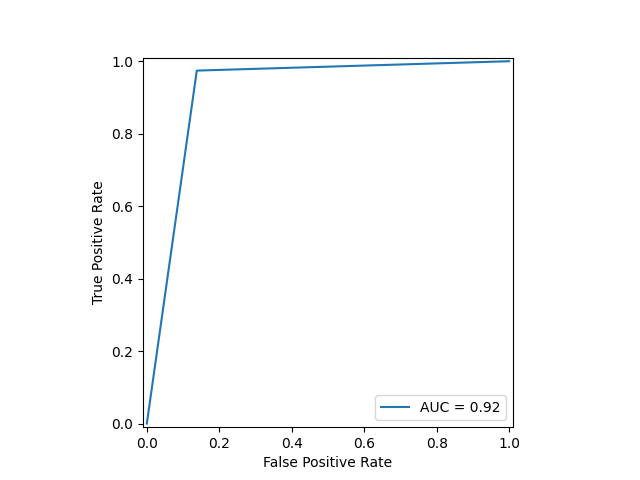
\includegraphics[width=3.5cm]{Curve_ANN.png}}
  \quad
  \subfloat{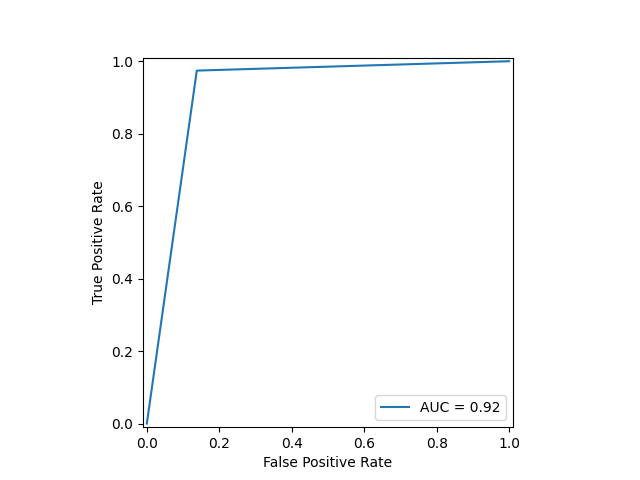
\includegraphics[width=3.5cm]{Curve_ANN.png}}
  \quad
  \caption{The receiver operating curves (ROC) of the ANN model recorded on both datasets}
\end{figure}

Table 3 shows a comparaison between our proposed method and the method covered in previous sections. Our proposed machine learning model has outperformed all other models while scoring an accuracy of 92\% on the AntiCP 2.0 dataset and 91\% on the CancerPPD dataset. 

\begin{table}[h!]
  \centering
  \resizebox{\columnwidth}{!}{
    \begin{tabular}{||c c c c||}
      \hline
      Study & Dataset(s) & Metic(s) & Results \\
      \hline \hline
      Yan et al.\cite{yuan2023prediction} & CancerPPD & accuracy & 79.9\%  \\
      Agrawal et al. \cite{agrawal2021anticp} &AntiCP main & accuracy& 77\% \\
      Schaduangrat et al. \cite{schaduangrat2019acpred} & APD2 & MCC & 91\%\\
      \textbf{proposed method} & AntiCP 2.0 \& CancerPPD & accuracy & \textbf{92\%} 91\%\\
      \hline
    \end{tabular}}
  \caption{A comparaison between our proposed method and other studies}
  \label{table:2}
\end{table}


\section{Conclusion}
This study introduced a machine-learning pipeline to detect ACP. The best performance is recorded using the proposed artificial neural network.

In further steps of the study, we suggest using long short-term memory (LSTM) and one-dimensional convolutional neural networks (1D CNN) to directly classify peptide embeddings.


\bibliographystyle{abbrv}
\bibliography{refs}

\end{document}

